\documentclass[11pt,a4paper]{article}
\usepackage[left=2cm,text={17cm,25cm},top=2.5cm]{geometry}
\usepackage[T1]{fontenc}
\usepackage[english]{babel}
\usepackage[utf8]{inputenc}
\usepackage{url}
\usepackage{graphicx}
\usepackage{pdfpages}
\graphicspath{ {img/} }

\begin{document}

\begin{center}
	\LARGE{Data Communications, Computer Networks and Protocols -- Project}\\
	\large{Brno University of Technology}
	\vspace{0.5cm}

	Petr Stehlík <xstehl14@stud.fit.vutbr.cz>

	\vspace{0.2cm}

	\today

\end{center}

\section{Assignment}
The task in hand was to create whitelisting of detected alerts for the NEMEA system with connection to the visualization part in Liberouter GUI. Whitelisting is only a partial feature which was needed. Because of this the project aims to create an improved version of reporting modules of the NEMEA system. The work is based on modification and improvement of a shared python module called \textit{report2idea}.

The goal of the new version is to enable advanced alert filtering that is performed according to global configuration file. Besides just filtering, users can specify a list of \textit{actions} that are executed when the given \textit{condition} is fulfilled and a list of \textit{elseactions} that are executed when the \textit{condition} is not fulfilled.

This document describes the analysis and implementation of such expansion while defining a format for configuration which is the cornerstone of the whole system.

\section{Analysis}
\subsection{System Architecture}

The current reporters' architecture is modular and easily expandable. Each reporter module imports common Python module called \textit{report2idea} that implements core functionality of handling reported alerts. \textit{report2idea} connects to the TRAP\footnote{http://nemea.liberouter.org/trap-ifcspec/} interface, receives alerts and performs desired actions. Currently it allows for storing IDEA formatted alerts into MongoDB, Warden system and resending them via TRAP interface. These options depend on arguments passed to the reporter on start up.

The new architecture expands \textit{report2idea} module where on startup a YAML configuration file is loaded, checked and parsed by \textit{report\_config} module. When an alert is received it's matched against rules specified in the configuration and else/actions are performed (more about this in section \ref{confdesign}).

\textit{report\_config} uses Mentat Filtering\footnote{The lead creators are Jan Mach, Pavel Kácha and Andrea Kropáčová} module to parse conditions in rules and match alerts against them. Mentat internally uses its own module \textit{jpath} to traverse paths in dictionaries which is used in conditions to retrieve values from an alert.

\begin{figure}[ht]
    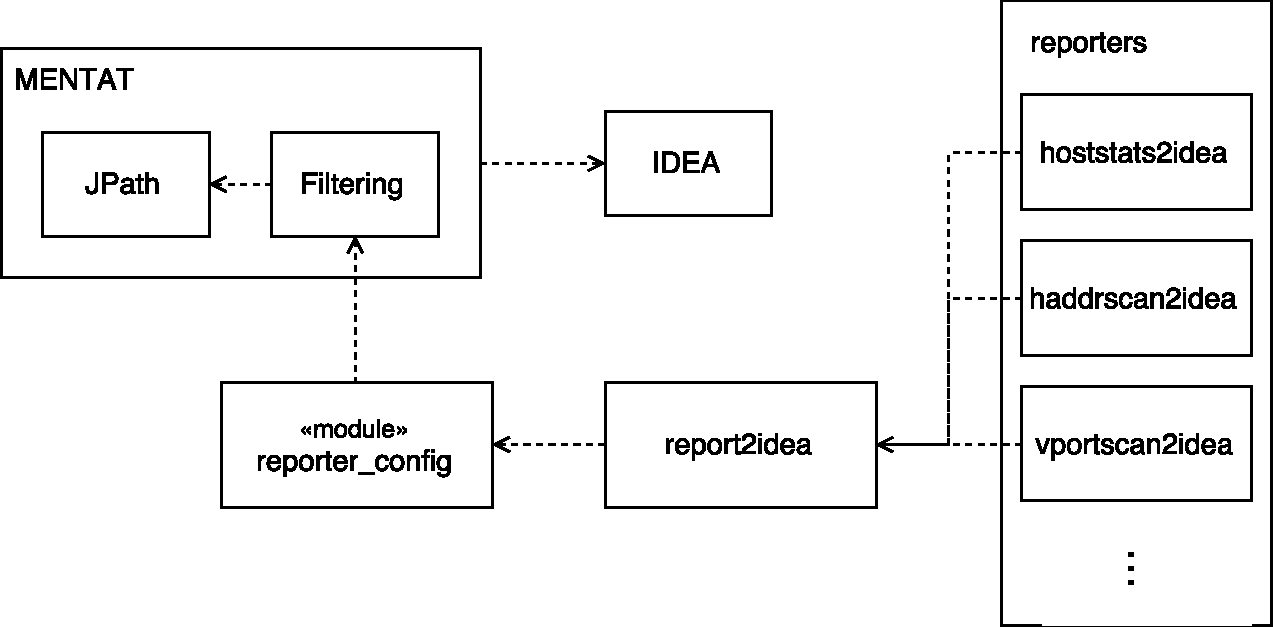
\includegraphics[width=0.65\linewidth]{schema.pdf}
    \centering
	\caption{New \textit{report2idea} expanded architecture}
    \label{schema}
\end{figure}

\subsection{Configuration Design}
\label{confdesign}
The configuration is divided into several parts: rules, address groups, custom actions and actions. Each part will be described in detail. The full example configuration can be seen at \ref{configfile}.

\subsubsection{Rules}
Each rule is composed of \textit{ID}, \textit{condition}, \textit{actions} and \textit{elseactions} which is an optional item. The list of rules is ordered by its numeric ID and evaluated in that order.

Filtering condition consists of unary and binary operations, constants and JSON paths that are parsed by the Mentat Filtering module. When an alert meets the condition, list of actions is performed in specified order. If a list of elseactions is defined and the filtering condition is not met this list of actions is performed.

\subsubsection{Actions}
Each rule specifies a list of \textit{actions} and optionally \textit{elseactions} that are of two types: implicit and custom. Currently the only implicit action available is to \texttt{drop} the alert which will immidiatelly stop processing it. This action mustn't be specified in custom actions.

The \texttt{custom\_actions} is a list of actions identified by ID string key -- this identifier is used to reference an else/action in a rule. Each custom action must specify its type. Currently available types of custom actions are as follows:

\begin{itemize}
		\label{actions}

	%\item{warden}
	%	\begin{itemize}
	%		\item{}
	%	\end{itemize}
	\item{file -- store alert into file}
		\begin{itemize}
			\item{dir[boolean] -- if set to \texttt{False} each alert is stored in separate file, otherwise it is appended to specified file}
			\item{path[string] -- path to file/folder respectively to \texttt{dir} option}
		\end{itemize}
	\item{email -- send alert via email}
		\begin{itemize}
			\item{to[string] -- recipient email address}
			\item{subject[string] -- subject field}
		\end{itemize}
	\item{mongo -- store alert to MongoDB}
		\begin{itemize}
			\item{host (optional)[string] -- MongoDB instance host (defaults to \textit{localhost}}
			\item{port (optional)[number] -- MongoDB instance port (defaults to \textit{27017}}
			\item{db[string] -- database name}
			\item{collection[string] -- collection name}
			\item{username (optional)[string] -- MongoDB username (needed in case of enabled authentication)}
			\item{password (optional)[string] -- MongoDB user's password (needed in case of enabled authentication)}
		\end{itemize}
	\item{mark -- add/modify value in alert}
		\begin{itemize}
			\item{path[JSONPath] -- JSONPath in alert, if non-existent it is created}
			\item{value[string] -- value to add}
		\end{itemize}
	\item{trap -- send the message via TRAP IFC if it is opened for the reporter, otherwise the action takes no effect}

\end{itemize}

\subsubsection{Address Groups}

Condition might refer to a named list of addresses. This feature extends Mentat Filtering. Each address group is identified by its string ID. Each address group must specify a file or a list of IP addresses/subnetworks. An address group file is a list of IP addresses/subnetworks separated by newline.

\section{Implementation}

The new report2idea takes \texttt{config} argument which specifies path to a configuration file. This value is passed to an instance of Config class. The file is loaded and parsed by PyYAML module to dictionary. Afterwards Mentat Filtering is initialized in order to parse rules conditions. Next address groups are parsed. Depending on given configuration it can load and parse file address group which translates it to a list.

With address groups parsed it continues to parse custom actions. Each action is recognized by its type and an Action class is instantiated accordingly. This enables to create unlimited number of types and its actions in the future. Each action takes different arguments as specified in \ref{actions} and implements \texttt{run} method which performs desired action. Right after custom actions parsing the implicit drop action is added as well.

The last part on initialization procedure is rules parsing. Each rule takes its dictionary representation, list of actions, list of address groups and optionally a Mentat Filtering instance (if not given each rule creates its own instance). Rule then parses its condition -- finds all occurrences of address groups IDs and replaces them with a list of IP addresses/subnetworks and then parses the condition via Mentat Filtering. Finally, the rule links all its specified actions and elseactions with actions available in custom actions and in implicit actions.

Afterwards the report2idea \texttt{Run()} function starts to receive alerts from TRAP interface. Each received alert is converted to IDEA message, matched against available rules and the list of actions or elseactions is performed accordingly. This continues until TRAP interface or the reporter is terminated.

The visualization part of whitelisting is done via a mark action (as shown in \ref{configfile} in \textit{markwhitelisted} custom action). It adds \texttt{\_CESNET.Whitelisted} flag to the alert with boolean value. Afterwards Liberouter GUI NEMEA Events module (it displays alerts saved to MongoDB) looks for such flag and if set to True, hiding the whitelisted alerts or visually differentiating them from non-whitelisted alerts as seen in \ref{before}.

\section{Conclusion}
Advanced alert filtering and its configuration was designed and implemented successfully. Only minimal changes were needed in reporters (the only change is in arguments passed to the reporter). During the development of the it a bug in Mentat Filtering was found and fixed.

Further work will focus on autonomous recognition of configuration and addressgroups changes which will trigger reload and parsing of the updated configuration, deeper integration with NEMEA system and Liberouter GUI which will enable to edit the configuration and address groups comfortably via web interface with minimal margin for error.

The whole project is available on Github in Nemea-Framework repository \footnote{https://github.com/CESNET/Nemea-Framework/tree/reporter-config/pycommon} and a Python package is being prepared in order to be easily deployable.
\newpage

\section{Annexes}
\subsection{Example Configuration File}
\label{configfile}

%\begin{lstlisting}[language=yaml]
\begin{verbatim}
custom_actions:
- id: mongo1
  type: mongo
  host: localhost
  db: nemeadb
  collection: alerts
- id: marktest
  type: mark
  mark:
    path: Test
    value: 'FooBar'
- id: markwhitelisted
  type: mark
  mark:
    path: _CESNET.Whitelisted
    value: 'True'
- id: savefile
  type: file
  dir: true
  path: "/var/log/nemea/events"
addressgroups:
- id: main_whitelist
  file: "/etc/nemea/reporters/whitelists/whitelist1"
- id: whitelist2
  list:
  - 1.1.0.0/24
  - 1.2.3.4
rules:
- id: 1
  condition: Source.IP4 in main_whitelist or Target.IP4 in main_whitelist
  actions:
  - markwhitelisted
  - mongo1
  - drop
  elseactions:
  - marktest
  - savefile
  - mongo1
- id: 2
  condition: >
	   Node.SW == 'detector1' and
	   Category == 'Recon.Scanning' and
	   Target.IP4 in whitelist2
  actions:
  - marktest
- id: 3
  condition: Source.IP4 == whitelist2
  actions:
  - drop
- id: 4
  condition: Node.SW in ['detector1', 'detector2']
  actions:
  - savefile
  - drop
\end{verbatim}
%\end{lstlisting}

\subsection{Whitelisting visualization}
\begin{figure}[ht]
    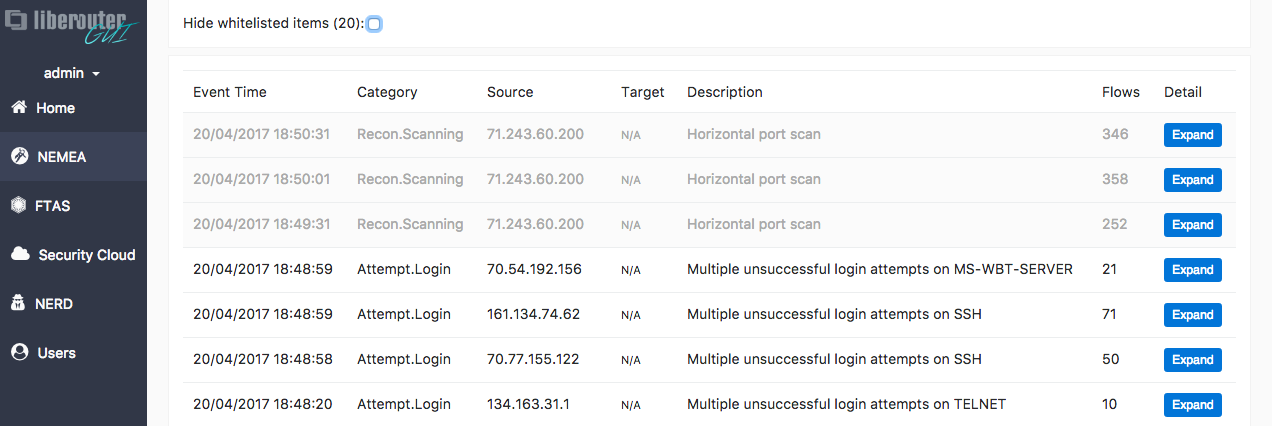
\includegraphics[width=\linewidth]{before.png}
    \centering
	\caption{Visually separated whitelisted alerts in Liberouter GUI NEMEA Events}
    \label{before}
\end{figure}
\begin{figure}[ht]
    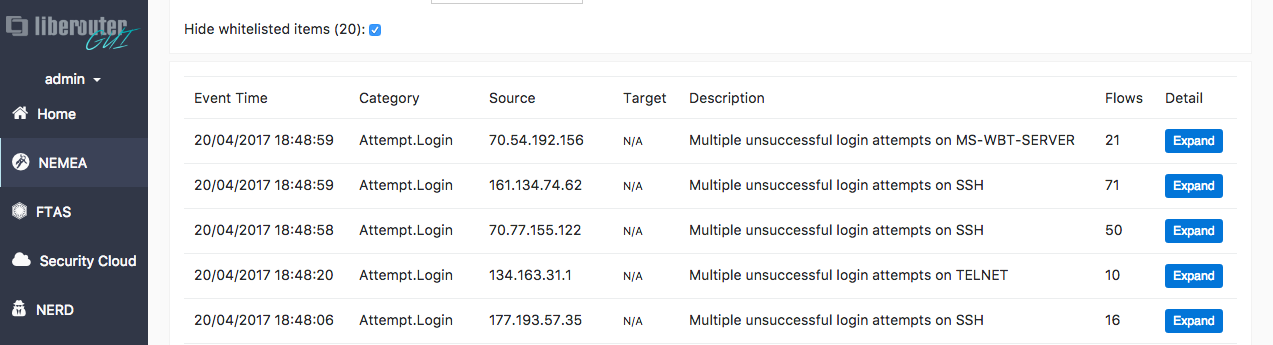
\includegraphics[width=\linewidth]{after.png}
    \centering
	\caption{Hidden whitelisted alerts in Liberouter GUI NEMEA Events}
	\label{after}
\end{figure}

\end{document}
